\documentclass[a4paper]{article}

% Load the VUB package.
% This has many options, please read the documentation at
% https://gitlab.com/rubdos/texlive-vub
\usepackage{vub}
\usepackage[english]{babel}

% Some highly suggested packages, please read their manuals.
\usepackage{hyperref}
\usepackage{float}
\usepackage{xcolor}
\usepackage{listings}

\usepackage{xparse}
\usepackage{cleveref}
\usepackage[natbib, style=ieee]{biblatex}
\usepackage{csquotes}
\addbibresource{bibliography.bib}
\setlength\parskip{\baselineskip}
\definecolor{darkred}{rgb}{0.6,0.0,0.0}
\definecolor{darkgreen}{rgb}{0,0.50,0}
\definecolor{lightblue}{rgb}{0.0,0.42,0.91}
\definecolor{orange}{rgb}{0.99,0.48,0.13}
\definecolor{grass}{rgb}{0.11, 0.53, 0.17}
\definecolor{pink}{rgb}{0.97,0.15,0.45}
\definecolor{backcolour}{rgb}{0.95,0.95,0.92}

\newcommand{\secref}[1]{\autoref{#1}.}

\lstdefinestyle{mystyle}{
  basicstyle=\ttfamily,
  backgroundcolor=\color{backcolour},   
  commentstyle=\color{darkgreen}\itshape,
  keywordstyle=\color{blue}\bfseries,
  stringstyle=\color{red},
  showspaces=false,                
    showstringspaces=false,
    showtabs=false,
    breakatwhitespace=false,         
    breaklines=true,                 
    captionpos=b,                    
    keepspaces=true,                 
    numbers=left,                    
    numbersep=5pt,
}

\lstset{language=Python, style=mystyle}
\title{Delivering systems with Stork}
\pretitle{\flushleft{Bachelor thesis submitted in partial fulfillment of the requirements for the degree of bachelor of science: Computer Science}}
\subtitle{ A distributed computing deployment tool}
\author{Gérard Lichtert}
\date{\today}
\promotors{Promotors: Prof.\ Dr.\ Joeri de Koster and Prof.\ Dr.\ Wolfgang de Meuter. \and Advisor: Mathijs Saey}
\faculty{Sciences and Bio-Engineering sciences}

\begin{document}
\maketitle
\tableofcontents
\newpage
\raggedright{}


\section{Introduction}
In a world of electronics and machines where power consumption is always increasing, optimizing power consumption is becoming increasingly important. While electricity is expensive, the main reason lies in climate change. This is because the majority of our electricity production still comes from non-renewable sources, such as coal, oil, and gas \cite{owid-energy-mix}. These sources produce a lot of CO\textsuperscript{2}, and other greenhouse gases, which are the main contributors to climate change. While there is research being done to optimize energy generation, optimizing power consumption is becoming increasingly important. This means that we as programmers can also play a role in optimizing our programs to consume less energy.

In the world of computing, cloud computing is responsible for 1\% of the worldwide energy consumption \cite{cloudcomputingenergycrisis}. To make use of the cloud, we do not only need electricity to power the devices that provide cloud computing but also electricity to power the Internet, which also plays a significant role in energy consumption. This is because the Internet is the backbone of most if not all, communication between devices and applications. The amount of connected devices and applications keeps growing, which leads to higher network usage. Consequently, higher network usage also leads to higher energy consumption, which leads to a higher carbon footprint \cite{RATHEESH}. Higher network usage also requires better infrastructure to handle the increased data volume, which in turn also requires more energy \cite{datavolumeeffects}. To reduce the network load we need to look at the data that is being sent through the network and if we can reduce it.

Data is usually transported through the network for a few reasons. Sometimes it is to send data to a device to update local data, like a chat message that needs to be added to the chat, or a new email that needs to be downloaded. While often compressed, the data is used as-is, and thus cannot be further reduced. Other times, however, data is sent to be processed. This can potentially be optimized by applying the edge-computing principle. This means that (part of) the data that is originally meant for processing is processed locally first, potentially reducing the amount of data that needs to be sent after preprocessing it. Logically, the network load, and consequently the energy consumption, should be reduced. However, for a certain set of devices or applications, it could be optimal to pre-process the complete set of data prior to sending it over the network, while for another set of devices or applications, it could be optimal to send the data directly to the server. Sometimes, however, the optimal configuration could be a combination of the two. This gives rise to the question of how we can declare how certain data is processed, and where it is processed and on top of that change the where without much manual intervention. Moreover, we want this to be available in Python because it could be interesting for further data science\cite{datasciencelanguage} or AI applications, in which the language is known to be very popular. For this purpose, we introduce Stork.

Stork is a distributed computing deployment tool, written in Python that makes it possible to deploy distributed systems and try out different configurations regarding these systems. More concretely, it allows us to initialize the deployment of a distributed system, change the configuration of where certain parts of the distributed system are deployed in a declarative way and reverse the deployment.
\section{Background}
Before we discuss Stork, we need to discuss the goals that Stork should achieve and how. As mentioned in the introduction, we require a tool that allows us to declare where which data gets processed. This means that we need to be able to deploy parts of our program to different devices. Consequently, this means that our tool needs to work in the context of distributed systems. For this we need to choose a distributed computing paradigm that allows us to deploy our system in a distributed way, as well as change where parts of our programs reside. Next, we need to look at the available technologies and libraries in Python and choose the one(s) that best fit our needs. Let us begin with the distributed computing paradigm.
\subsection{Distributed computing paradigm}
\label{sec:distributedcomputingparadigm}
To start with distributed computing, we have to look for a suitable distributed computing paradigm that allows our system to be deployed from the cloud without much manual intervention, yet is able to do what we require it to do. There are several options, such as:
\begin{enumerate}
    \item Message Passing Interface (MPI)\cite{MPI}
    \item Remote Procedure Call (RPC)\cite{RPC}
    \item Shared Memory Model\cite{SMM}
    \item The Actor Model\cite{ActorModel}
\end{enumerate}
While each paradigm has their strengths and drawbacks, we will be using the Actor Model. An Actor is a computational unit which encapsulates its state and behavior, interacting with each other through asynchronous message passing. Each Actor has a mailbox, in which it receives these messages and processes them sequentially. Because of the message-based communication between Actors, we can easily decouple components, which in turn makes it easier to debug and test our systems. This is beneficial because distributed systems can quickly become very complex.

The encapsulation property of the Actor Model allows Actors to be very modular, as we can see each Actor as a separate unit that processes part of the data. More concretely, each actor will be responsible for processing a single part of the data. This allows us to easily move parts of the data processing pipeline from one device to another. This is important because we want to be able to change where which data gets processed without much manual intervention. Using an IoT system as a running example because IoT devices account for 50\% of networked device\cite{differentnetworkneedsiot}. It is possible to encapsulate the behavior of each sensor in an Actor, connect this with another Actor responsible for sending the data to a server where the data gets sent through a series of Actors that are each in turn responsible for processing a single part of the data, just like in figure \ref{fig:iotActorExample1}.
\begin{figure}[H]
    \centering
    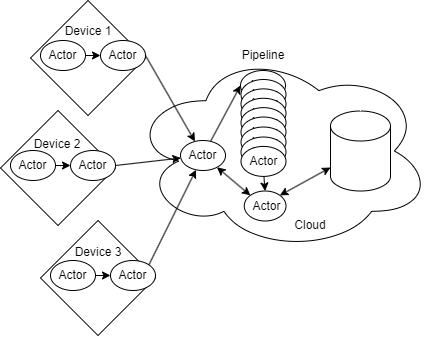
\includegraphics[width=0.65\textwidth]{iotActorExample1.png}
    \caption{An example of an IoT system using the Actor Model}
    \label{fig:iotActorExample1}
\end{figure}
Conceptually we should be able to move some of the Actors that process data from the pipeline to the IoT devices and place them before the the Actor that sends the data to the Server, as depicted in figure \ref{fig:iotActorExample2}. Achieving one of the possible configurations discussed in the introduction, without having to reprogram the entire system.
\begin{figure}[H]
    \centering
    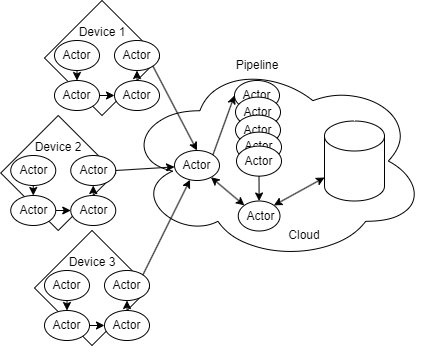
\includegraphics[width=0.65\textwidth]{iotActorsMoved.png}
    \caption{An example of an IoT system where some of the Actors that process data are moved to the IoT devices}
    \label{fig:iotActorExample2}
\end{figure}
While it is technically possible to achieve modularity in MPI, RPC, and the Shared Memory Model, due to the tight coupling of those models, it is harder to achieve. This is because the state and behavior of the system are not encapsulated in a single entity, but rather spread across the entire system. This makes it harder to move parts of the system around.
\subsection{Implementing Actors in Python}
When using Stork to deploy distributed systems and trying out different configurations, we need to create Actors that can be deployed by Stork. However, before we can discuss how to use Stork, we need to discuss how to implement Actors in Python. Since Stork is built with Thespian, a Python Actor library, we will be using Thespian to implement our Actors. Consequently Stork only works with Thespian Actors. To create an Actor one must create a class that inherits from a Thespian Actor class. Furthermore this Actor must at least implement the \lstinline{receiveMessage} method or equivalent, depending on the Actor class that is extended. As mentioned in \secref{sec:distributedcomputingparadigm}, Actors communicate through asynchronous messaging. This means that when the Actor receives a message it will call the \lstinline{receiveMessage} method. An example of an Actor is given below
\begin{lstlisting}[language=Python, caption=Actor example, label=lst:actor]
from thespian.actors import Actor

class HelloWorld(Actor):

    def receiveMessage(self, message, sender):
        if message == "are you there?":
            self.send(sender, "Hello World! back")
\end{lstlisting}
\section{Stork}
As mentioned in the introduction, Stork is a distributed computing deployment tool, written in Python that makes it possible to deploy distributed systems and try out different configurations regarding these systems. As perviously mentioned there are some implications when using Stork, as it is built on Thespian, a Python Actor library. This means that Stork only works with Thespian Actors. Stork provides the following features:
\begin{enumerate}
    \item Initializing the distributed system, allowing Actors to be spawned on the declared devices.
    \item De-initializing the distributed system, removing all Actors from the declared devices.
    \item Delivering an Actor class to the devices, allowing the Actor to be spawned on the device. This comes in two variants.
\end{enumerate}
\subsection{Initializing the distributed system}
When the user of Stork wants to initialize the distributed system, the user has to declare which devices take part of the distributed system. More importantly, Stork needs to know from which of these devices the distributed system should be initialized. This is because Thespian requires a leader device, to which the other devices register themselves to. Stork in turn uses this leader device to keep track of the registered, or remote devices, and spawn Actors on the remote devices and the leader device. It is expected that the user uses this method prior to deploying the user defined Actors. Otherwise the user defined Actors cannot be spawned.
\begin{lstlisting}[language=Python, caption=Initializing the distributed system, label=lst:init]
import Stork

if __name__ == "__main__":
    # First we declare a list of the host names of the devices that have to be part of our distributed system
    devices = ["server@vub.ac.be","device1", "device2", "device3"]
    # Then we call the distributeSystem method, with the leader device being the first host name in the list of devices.
    Stork.distributeSystem(leader=devices[0], convention=devices)
\end{lstlisting}
It is expected that the user calls this method on the leader device, because it is expected that the leader device has access to the other devices.

Alternatively, a user of Stork can instead of declaring the devices in a list, declare them in a dictionary with the keys as the host names and a list of properties as the value. This way the user can declare the capabilities of the devices, which can be used to spawn Actors on the devices that have the requested capabilities.
\begin{lstlisting}[language=Python, caption=Initializing the distributed system with capabilities, label=lst:initcap]
import Stork

if __name__ == "__main__":
    # Just like before we declare our devices, but this time in a dictionary with the host names as keys and the capabilities as values.
    devices = {
        "server@vub.ac.be" : ["server", "database"],
        "device1" : ["sensor"],
        "device2" : ["sensor"],
        "device3" : ["sensor"]
    }
    Stork.distributeSystem(leader=devices.keys()[0], convention=devices)
\end{lstlisting}
Again, it is expected that the user calls this method on the leader device, because it is expected that the leader device has access to the other devices.
\subsection{De-initializing the distributed system}
De-initializing the distributed is the opposite of initializing the distributed system. This is necessary because when the user is done with the distributed system, all processes must be stopped. Since all processes of the Actors are running on the background on the devices declared when calling \lstinline{distributeSystem}, Stork creates a connection with the devices and runs a script to end all Actor related processes. Just like \lstinline{distributeSystem}, it is expected that the user calls this method on the leader device.
\begin{lstlisting}[language=Python, caption=De-initializing the distributed system, label=lst:deinit]
import Stork

if __name__ == "__main__":
    Stork.undistributeSystem()
\end{lstlisting}
\subsection{Delivering an Actor class to the devices}
Now that the methods to initialize and de-initialize the distributed system have been discussed, we can discuss how to distribute the Actors. Whenever the user wants to spawn an Actor on a device, the user can use two different methods to spawn the given Actor class. Stork provides two methods for this: \lstinline|deliverActor| and \lstinline|deliverOrActor|. However, these methods must be called within an Actor. This is because Stork uses the Actor to communicate internally, that an Actor must be spawned on a certain device.

The \lstinline{deliverActor} method takes the Actor calling the method as an argument and a list of capabilities as a second argument. The list of capabilities is used to determine on which devices the Actor should be spawned. Taking a look at the example from listing \ref{lst:initcap}, if we want to spawn an actor on all the devices with the capability \enquote{sensor}, we can use \lstinline{Stork.deliverActor(self, ActorClass, ["sensor"])}. However, if we only want to spawn the Actor on one of the sensors, we can use \lstinline{Stork.deliverActor(self, ActorClass, ["device1"])}, or \lstinline{Stork.deliverActor(self, ActorClass, ["sensor", "device1"])}. Regardless, \lstinline{deliverActor} will spawn the Actor on all devices that have the all requested capabilities.
\vfill
\begin{lstlisting}[language=Python, caption=Delivering an Actor, label=lst:deliverActor]
import Stork
from thespian.actors import Actor

class Pong(Actor):

    def receiveMessage(self, message, sender):
        self.send(sender, "pong")

class Ping(Actor):

    def receiveMessage(self, message, sender):
        if message == "spawn":
            Stork.deliverActor(self, Pong, ["sensor"])
\end{lstlisting}

Now that Stork spawned Actors on all the devices that have the \enquote{sensor} capability, how do we interact with them? As mentioned in \secref{sec:distributedcomputingparadigm}, Actors communicate through asynchronous messaging. In thespian this means that when a message is sent from an Actor to another Actor, it will never receive a return value. \lstinline|deliverActor| and \lstinline|deliverOrActor| are no exceptions to this rule, since they work in a similar manner. However, when an Actor sends a message to another Actor it can send a message back. Consequently, the user of Stork needs to extend the \lstinline|receiveMessage| method to handle the message that Stork sends to the Actor calling the delivery methods. This message contains the references to the Actors that have been spawned. Once the Ping Actor has the references it can interact with the spawned Actors in a similar manner as it would with other thespian Actors.

Stork provides a Class to easily encapsulate the message that is sent to the Actor calling the delivery methods. This class is called \lstinline||


\section{Implementing Stork}
\section{Conclusion}

\subsection{Technologies and libraries}
As mentioned when choosing the programming language of implementation, Python offers two Actor Model libraries. Pykka and Thespianpy. Setting Pykka and thespian next to each other and comparing them yields the following results:
\subsubsection{Pykka}
Quoting the documentation of the library: \enquote{Pykka is a Python implementation of the actor model. The actor model introduces some simple rules to control the sharing of state and cooperation between execution units, which makes it easier to build concurrent applications.} However, reading further down in the documentation we see that Pykka has some shortcomings, as it does not support linking actors, supervisors, or supervisor groups. It does not support communicating with actors running on other hosts, nor does it come with a set of predefined message routers. This would mean that we have to implement this ourselves, particularly the communication between actors running on other hosts. This is important because we are building a distributed system after all, and we need to be able to communicate between different hosts. Notably it does have \(\approx 1200\) stars on Github, which comparing it to Thespianpy, is more. Meaning that it is more popular than Thespianpy and thus has a larger community using it.
\subsubsection{Thespianpy}
The documentation states that: \enquote{Thespian is a Python library providing a framework for developing concurrent, distributed, fault-tolerant applications. It is built on the Actor Model which allows applications to be written as a group of independently executing but cooperating "Actors" which communicate via messages. These Actors run within the Actor System provided by the Thespian library.} More importantly, Thespianpy allows us to run Thespian on different hosts, while internally handling the messaging between actors, providing an out-of-the-box solution for Actor communication between different hosts. This means that when using the Thespian library, we do not have to implement the communication between actors running on different hosts. It also means that we can user the built-in communication to declare where which data gets processed. However, it only has \(\approx300\), which is significantly less than Pykka.
\subsubsection{Our verdict}
While Pykka is more popular than Thespianpy, it does not support communication between actors running on different hosts. As this is a crucial feature for distributed computing, we choose Thespianpy.
\section{A deep dive into Thespianpy}
Now that we have chosen the technologies and libraries that we will be using to build Stork, we first need to design the tool to see if we need anything else. Since this tool will be built using Thespian, we will heavily rely on its provided features. This gives rise to a few questions:
\begin{enumerate}
    \item How do we deploy the system using Thespianpy?
    \item How can we declare where which data gets processed, using Thespianpy?
\end{enumerate}
Looking at the Thespianpy documentation, it states that we can deploy a system by starting an Actorsystem on a device. This Actorsystem will then manage the local Actors and their communication for us. Consequently, this also means that we will have to spin up an Actorsystem on each device, if we want Actors to live on those devices. Perhaps worth mentioning is that Thespianpy Actorsystems have different communication protocols, from which we can choose. However, the recommended setting for distributed systems is to use 'multiprocTCPBase', which lets Actors run on their own separate process, creating a truly asynchronous system. This also means that the communication method between Actors is TCP. Another option is to user 'multiprocUDPBase', which uses UDP as the communication method. Consequently, there will be no guarantee that the messages will be delivered, as this is a characteristic of UDP. The other options, multiprocQueueBase and simpleSystembase do not support multiple systems and cannot be used for inter-system communications, respectively. The configuration that will be used for Stork is 'multiprocTCPBase'. Prior to continuing the deployment of the Actorsystems across several devices, we need to introduce some important concepts regarding the Actors, Capabilities and Conventions.

As asked before, how can we declare where which data gets processed in our distributed system, using Thespianpy? As mentioned in section 2.1, where the distributed computing paradigm was chosen, we can leverage the modularity of the Actor Model to split our data processing pipeline in small enough segments. Ideally each segment would be responsible for processing one part of the data, obtaining more flexibility for moving parts around. More concretely, each segment in our pipeline would be encapsulated by an Actor, making each Actor responsible for processing a part of the data. This is how we declare which data gets processed, but how do we declare where our data gets processed?

Logically, this would mean that the Actor processing a specific part of the data should be placed on the device where we want that part of the data processed. While thespianpy does support the creation of Actors on remote hosts and their communication, it is not evident as to how the same Actor is supposed to be spawned on different hosts. Let me explain: Thespian has a built-in mechanism to allow Actors to be spawned on a remote host however, this is not by declaring the Actor to be spawned on said host. Instead, Thespianpy allows for restricting an Actor to be spawned on certain hosts, without the guarantee that the Actor is spawned on the host that we want the Actor to be spawned on. This built-in mechanism is called 'Capabilities', which allows an Actorsystem to be spun up with certain capabilities, and an Actor to be spawned only on the Actorsystem where those capabilities are present. Furthermore, Thespianpy will always spawn an Actor on the first Actorsystem within the distributed system that has the required capabilities. Consequently, this does not guarantee that we can spawn the same Actor on different devices, as more often than not, Thespianpy will spawn the same Actor multiple times on the same Actorsystem. This follows from the fact that the same Actorsystem will often be the first one where the Actor is able to spawn. This is a problem, because in a scenario where we have several sensors, and we want to spawn an Actor on all the sensors, we won't be able to guarantee that the Actor is spawned on all the sensors.

Worth mentioning is that Thespianpy allows for Actor creation by invoking a method on the local Actorsystem. However this only works when the capabilities that the Actor requires to be spawned on the local Actorsystem are present on the local Actorsystem. If they are not, the program crashes. So how are we supposed to spawn an Actor on a remote device? Well while we cannot spawn an Actor on a remote machine using the Actorsystem, we can using an Actor. This means we would first have to create an Actor locally and use that Actor to spawn an Actor with incompatible capabilities with that of the local Actorsystem, to spawn it remotely.

At a first glance, Thespianpy seemed to have a method, that when called from an Actor, to spawn another Actor, we could pass the capabilites that the Actorsystem is required to have to be able to spawn the Actor. Say we have a distributed system with three devices, A, B, and C. We want to spawn an Actor that pre-processes data on devices B and C. We could let the Actorsystems on those devices have a common capability, say 'device\_B\_C'. Now in theory, if we give each Actorsystem its host name as a capability as well, we should be able to guarantee that the Actor is spawned on devices B and C if we pass the 'device\_B\_C' capability as well as the hostname of the remote device where the Actor should be spawned. However, this is not the case. When testing this method, while Thespianpy would interpret the common capability correctly, it ignored the hostname capability. Meaning that we still did not have the guarantee that the Actor would spawn on both B and C and not twice on either device. Presumably, the Capabilities are not processed in a way that the Actorsystem is required to have all declared Capabilities but rather only one of them.

Making another attempt at solving the problem distribution of Actors, let us try to exploit how Actorsystems are connected with each other. Actorsystems work by registering themselves to a convention leader. Meaning that an Actorsystem or rather the leader Actorsystem has to be spun op before the rest of the Actorsystems within the convention. While it works mostly internally and is hidden from the programmer, we can still get be informed of the Actorsystems registering to the convention leader. This is achieved by creating an Actor on the leader Actorsystem and invoking \textit{self.notifyOnSystemRegistrationChanges}. This method will tell the leader Actorsystem that the Actor subscribes itself to receive notifications about updates in the convention. It provides the Actor with notifications of registrations and de-registrations, as well as the admin address of the remote Actorsystem as well as the capabilities of the remote Actorsystem. Note that the admin address of the remote Actorsystem is actually the address (or reference) to a top-level Actor of the remote Actorsystem, that manages the Actorsystem internally, not the the address or reference to the Actorsystem itself. This Actor is invisible to the user.

When working locally with Actors, and creating other Actors, we actually create references, or addresses of those Actors, with which we can asynchronously send messages to. Knowing this, theoretically it could be possible to use the provided admin address of the remote Actorsystem to create Actors on the remote Actorsystem. We could do this by sending it a message to spawn an Actor. However, that is not the case. This because if we wanted the remote Actor to be able to spawn Actors, we would first have to implement a method in that Actor that would allow the Actor to interpret the sent message that tells it to spawn an Actor and send the created reference back. Since the remote Actor is invisible to the user, we cannot implement this method, leaving us with a way to send messages to the remote Actor but no way to for it to interpet it. We are yet again left with no solution. However, not all is in vain because we can still use the capabilities to our advantage to denote certain properties of the device on which the Actorsystem resides. We can keep track of the devices that have certain capabilities and then use this information to know where to spawn the Actors. However, this is not yet a complete solution.

What if instead of trying to get references to the remote Actorsystems to the leader Actorsystem, we get the reference of an Actor which resides in the leader Actorsystem to the remote Actorsystem? After all, we do know that with the Capabilities feature, we can restrict an Actor to be spawned on an Actorsystem. More concretely, we can force a remote Actorsystem to spawn an Actor locally, that spawns an Actor that can only be spawned in the leader Actorsystem. This way we can get a reference to the leader Actorsystem, and communicate to that Actor the reference of the Actor to further interact with it as needed. For example for spawning other Actors. Will this work? Not always sadly. While Thespianpy's documentation states that when we spawn an Actor multiple times on the same system it will try to reuse the same Actor, this is not always the case. Meaning that if we create an administrative Actor on the convention leader to be notified about remote systems, and force remote systems to spawn the same adminstrative Actor (which will then be spawned on the convention leader because of its capability restriction) it won't always reference the initially created administrative Actor. Luckily for us there is a way to force Thespianpy to reuse the same Actor. This is done by using a global name for the Actor. This way, when an Actorsystem tries to spawn the administrative Actor, it will first look for a global reference to it. Only if it is not found, does it create a new one. This way we can guarantee that the same administrative Actor is referenced by all remote systems.

What does this mean for Stork? It means that there are some implications when deploying Actorsystems, as we firstly need to spin up an Actorsystem on the convention leader, as well as create the administrative Actor, which should have a global name, as well as be registered to get notifications about convention updates. Furthermore, we need to spin up Actorsystems on the other devices, that create a local Actor that tries to create the administrative Actor, but instead get a reference to the already existing one on the convention leader, while registering themselves as a reference to the convention leader. This reference can later be used for spawning other Actors on the remote devices. With the help of the administrative Actor, that keeps track of the capabilities of remote Actorsystems, it can spawn Actors on the remote Actorsystems by sending a message that invokes a method to spawn the declared Actor. This way we can, for example tell the administrative Actor to spawn an Actor on all remote Actorsystems with the capability "Sensor", which would spawn an Actor on all devices that have the capability "Sensor".

This implies that Stork requires two programs. One to deploy the Actorsystem on the convention leader as well as spawn the administrative Actor, and one to deploy the Actorsystems on the other remote devices, as well as spawn their respective registrator Actors. However, to run these programs we need to create a connection with the remote devices and run these programs. This can be done by using SSH, which is a secure way to connect to the remote devices. While it probably is not an issue to do this in small distributed systems, manually SSH'ing to 30 different devices in a large distributed system is not ideal. This means that we require something to automate this process.

\section{Automating the deployment}
When automating deployments, Infrastructure as Code (IaC) is often a topic that comes up, as it allows us to automate the process of deploying infrastructure. For IaC we have several options, as we can use several tools and libraries to automate the deployment. Some of the most popular tools are:
\begin{enumerate}
    \item Ansible
    \item Chef
    \item Puppet
    \item SaltStack
    \item Terraform
    \item CFEngine
    \item Fabric
\end{enumerate}
\printbibliography
\end{document}
